% $Id: TimeMgr_obj2.tex,v 1.1 2002/08/18 22:43:36 eschwab Exp $

%\section{Object Model}

Figure 2 shows the typical usage (instantiantion) of the Time Manager
within an application.  First, a calendar is created.  Then, time intervals
and time instants are created for clock usage and initialized as a time step,
start time, stop time and current time.  Similarly, a time interval and time 
instants are created and initialized for alarm usage.  Next, alarms are
created and intialized with the appropriate previously created time interval
and time instants.  Finally, a clock is created and initialized with its
corresponding time instants and time interval.  The clock is also associated
with the previously created calendar and alarms.  The clock is then ready
for timestepping and alarm checking.

\begin{center}
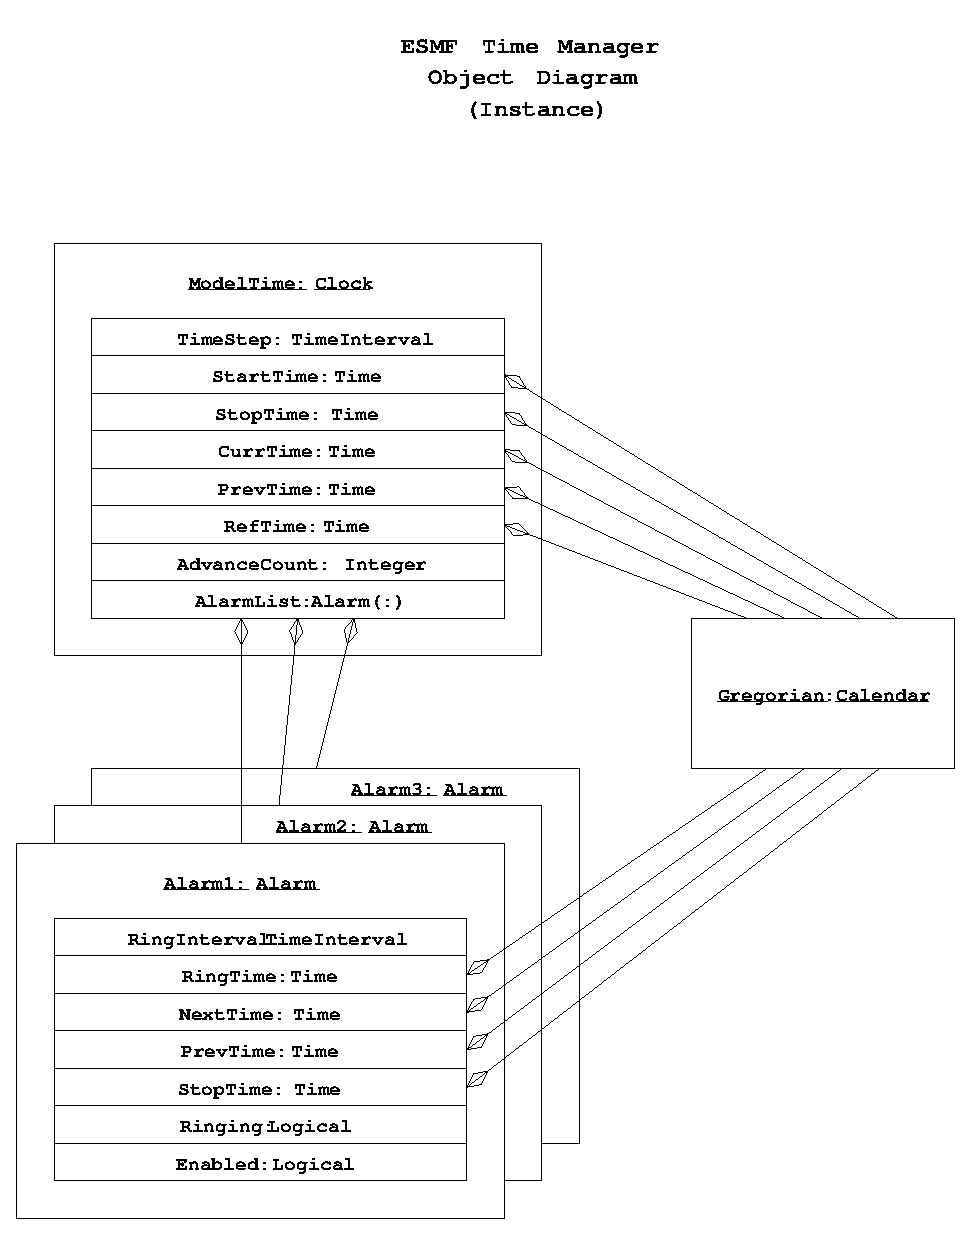
\includegraphics{TimeMgrObject.EPS}
   
Figure 2.  ESMF Time Manager Object Diagram
   
\end{center}
